%!TEX TS-program = xelatex
%!TEX encoding = UTF-8 Unicode

\documentclass[a4paper, oneside, british]{memoir}
\usepackage[datesep=/]{datetime2}

\usepackage{hyperref}
\PassOptionsToPackage{hidelinks}{hyperref}
\hypersetup{pdfborder=0 0 0}

\usepackage[backend=biber, style=ieee]{biblatex}
\addbibresource{main.bib}

\usepackage{fontspec}
\newfontfamily{\cascadia}{cascadiacode}
\setmainfont{Arial}
\newfontfamily{\arial}{Arial}
\newfontfamily{\fauna}{FAUNA}[Path = fonts/, Extension = .ttf, UprightFont = *-THIN]

\usepackage{lastpage}
\usepackage{pgfplots}
\usepackage{geometry}
\usepackage{bookmark}
\usepackage{hyperref}
\usepackage{enumitem}
\usepackage{calc}
\usepackage{longtable}
\usepackage{graphicx}
\usepackage{wrapfig}
\usepackage{listings}
\usepackage{amsmath}
\usepackage{bytefield}
\usepackage{pdfpages}
\usepackage{tikz}
\usepackage{tabularx}
\usepackage{amsmath}
\usepackage{array}
\usepackage{titlesec}
\usepackage{varwidth}
\usepackage{bytefield}
\usepackage{siunitx}
\usepackage{hyperref}
\usepackage{graphicx}
\usepackage[table]{xcolor}
\usepackage{tcolorbox}
\usepackage{bm}
\usepackage{svg}
\usepackage{lipsum}
\usepackage{fontawesome5}

\pagestyle{empty}

% ======================================================================================
%                                         MISC
% ======================================================================================

\setlist[itemize]{noitemsep}
\setlist[itemize, 1]{itemsep=0.5em,align=parleft,left=0pt..1.5em, label={\Large\textbullet}}

% Set up SI units
\sisetup{group-separator = {,}} % Separate groups with comma (i.e. 1,000,000)
\DeclareSIUnit{\feet}{ft}       % Add custom non SI unit for feet 

% Date style to display only the year
\DTMnewdatestyle{yearonly}{%
    \renewcommand{\DTMdisplaydate}[4]{\number##1}
    \renewcommand{\DTMDisplaydate}{\DTMdisplaydate}
}

\SetLabelAlign{parright}{\parbox[t]{\labelwidth}{\raggedleft#1}} 

\newcounter{tblerows}
\expandafter\let\csname c@tblerows\endcsname\rownum

% Define \setdocname to store the document name
\newcommand{\setdocname}[1]{\def\docname{#1}}
\newcommand{\docname}{}

% Define \setsysname to store the system name
\newcommand{\setsysname}[1]{\def\sysname{#1}}
\newcommand{\sysname}{}

% Define \setorglabel to store the organisation label
\newcommand{\setorglabel}[1]{\def\orglabel{#1}}
\newcommand{\orglabel}{}

% ======================================================================================
%                                    HEADER/FOOTER
% ======================================================================================

% Remove chapter/section number from rightmark
\makepsmarks{ruled}{%
 \nouppercaseheads
 \createmark{chapter}{right}{nonumber}{}{}
 \createmark{section}{right}{nonumber}{}{}
}

% Make header/footer rules full headwidth
\makerunningwidth{ruled}{\headwidth}

% Header/footer rules
\makeheadrule{ruled}{\headwidth}{2\normalrulethickness}
\makefootrule{ruled}{\headwidth}{2\normalrulethickness}{-0.20in}

% Change header/footer text & logo (use odds for single side)
\makeoddhead{ruled}{\textbf{\docname}}{}{\textbf{\rightmark}}
\makeoddfoot{ruled}{\small \thepage/\pageref{LastPage}}{\small \orglabel}{\includesvg[width=100pt]{./img/logo.svg}}

% ======================================================================================
%                                      SECTIONING
% ======================================================================================

\newcommand{\unnumbered}[2]{%
 \expandafter\csname#1\endcsname*{#2}
 \phantomsection
 \addcontentsline{toc}{#1}{#2}
}

% Set margins
%\setlrmarginsandblock{1in}{1in}{*} 
\setlrmarginsandblock{1.25in}{1.25in}{*} 
\setulmarginsandblock{1.25in}{1.25in}{*} 
\checkandfixthelayout%

% Define length to dedent text from margin to header width
\newlength{\margindedent}
\setlength{\margindedent}{0.5\textwidth-0.5\headwidth}

% Section title format 
\titleformat*{\section}{\huge\bfseries}
\titleformat*{\subsection}{\Large\bfseries}
\titleformat*{\subsubsection}{\large\bfseries}

% Section number format
\renewcommand{\thesection}{\arabic{section}}
\renewcommand{\thefigure}{\arabic{section}.\arabic{figure}}
\renewcommand{\thetable}{\arabic{table}}
\renewcommand{\abstractname}{Introduction}

% Label figures within sections
\numberwithin{figure}{section}

% Numbering
\setsecnumformat{\csname the#1\endcsname\hspace{0.5in-\widthof{\csname the#1\endcsname}}}
\setsecnumdepth{paragraph}

% Indentation
\setsecindent{1\margindedent}
\setsubsecindent{1\margindedent}
\setsubsubsecindent{1\margindedent}

\setlength{\absleftindent}{0em}
\setlength{\absrightindent}{0em}

\renewcommand{\baselinestretch}{1.125} % Scale baselineskip length
\setlength{\parskip}{0.5em}            % Adjust paragraph spacing
\setlength{\parindent}{0em}

% ======================================================================================
%                                      LISTINGS
% ======================================================================================

\lstset{language=C++,
        basicstyle=\ttfamily,
        keywordstyle=\color{blue}\ttfamily,
        stringstyle=\color{red}\ttfamily,
        commentstyle=\color{lightgreen}\ttfamily,
        morecomment=[l][\color{magenta}]{\#},
        numbers = left,
        breaklines = true
}

% Suppress numbering
\let\origthelstnumber\thelstnumber
\makeatletter
\newcommand*\Suppressnumber{%
  \lst@AddToHook{OnNewLine}{%
    \let\thelstnumber\relax%
  }%
}

% Restore numbering
\newcommand*\Reactivatenumber{%
  \lst@AddToHook{OnNewLine}{%
   \let\thelstnumber\origthelstnumber%
  }%
}
\makeatother

% ======================================================================================
%                                          TIKZ
% ======================================================================================

\newenvironment{xcenter}
 {\par\setbox0=\hbox\bgroup\ignorespaces}
 {\unskip\egroup\noindent\makebox[\textwidth]{\box0}\par}

\usetikzlibrary{positioning,fit,calc,chains,matrix,arrows.meta,shapes.geometric,arrows,backgrounds}

\pgfdeclarelayer{subbackground}
\pgfdeclarelayer{background}
\pgfdeclarelayer{foreground}
\pgfsetlayers{subbackground,background,main,foreground}

\tikzstyle{square} = [regular polygon, regular polygon sides=4, draw=black, inner sep=0cm, align=center]

% Flowchart shapes
\tikzstyle{start} = [rectangle, rounded corners, minimum width=3cm, minimum height=1cm, text centered, draw=black, fill=green!30]
\tikzstyle{stop} = [rectangle, rounded corners, minimum width=3cm, minimum height=1cm, text centered, draw=black, fill=red!50]
\tikzstyle{process} = [rectangle, minimum width=3cm, minimum height=1cm, text centered, draw=black, fill=orange!80, text=white]
\tikzstyle{decision} = [diamond, minimum width=3cm, minimum height=3cm, text centered, draw=black, fill=blue!50, text=white]
\tikzstyle{arrow} = [thick,->,>=stealth, draw=blue, text=blue]

\tikzstyle{board} = [
  rectangle, dashed, very thick, rounded corners, 
  minimum width=1cm, minimum height=1cm, inner sep=0.25cm,
  draw=gray
]
\tikzstyle{group} = [
  rectangle, very thick, rounded corners, 
  minimum width=1cm, minimum height=1cm, inner sep=0.25cm,
  draw=gray, fill=gray!25
]
\tikzstyle{second_group} = [
  rectangle, dashed, very thick, rounded corners, 
  minimum width=1cm, minimum height=1cm, inner sep=0.25cm,
  draw=gray, fill=white!5
]

\tikzstyle{element} = [rectangle, rounded corners, text centered, draw=black, minimum width=2cm, minimum height=1cm, fill=white]

\tikzstyle{register} = [rectangle, rounded corners, text centered, draw=black, minimum width=3cm, minimum height=1cm, fill=white]
\tikzstyle{inout} = [trapezium, draw=black, minimum width=2cm, fill=white]

% Colours
\definecolor{bittersweet}{rgb}{1.0, 0.44, 0.37}
\definecolor{aquamarine}{rgb}{0.5, 1.0, 0.83}
\definecolor{lavender}{rgb}{0.9, 0.9, 0.98}
\definecolor{whitesmoke}{rgb}{0.96, 0.96, 0.96}
\definecolor{pastelred}{RGB}{242,220,218}
\definecolor{pastelgreen}{RGB}{216,227,192}
\definecolor{pastelyellow}{RGB}{254,242,205}
\definecolor{lightgreen}{RGB}{102,153,0}    %#669900

% ======================================================================================
%                                   TABLE OF CONTENTS
% ======================================================================================
\makeatletter
\renewcommand{\@pnumwidth}{-3em}
\renewcommand{\@tocrmarg}{-4em}
\makeatother
 
% Lengths
% -------------------------------------------------------------------------
% Defines the width of a section number in the ToC
\newlength{\tocsecnumwidth}
\setlength\tocsecnumwidth{10ex}

% Defines the standard width of a subsection number in the ToC
\newlength{\tocsubsecnumwidth}
\setlength\tocsubsecnumwidth{7ex}

% This is a useful shorthand for defining the indents of entry
% titles as offsets from the top level title indent
\def\tocentrytitleindent#1{\margindedent + \tocsecnumwidth + #1}
% -------------------------------------------------------------------------

\renewcommand*{\tocheadstart}{\vspace*{-1em}}
\renewcommand*{\aftertoctitle}{\vspace*{-0.5em}}
\setcounter{secnumdepth}{3}
\setcounter{tocdepth}{3}

% Make section trailing dots bold in ToC
\renewcommand{\cftsectionleader}{\bfseries\cftdotfill{\cftdotsep}}

% ToC title format
\renewcommand\contentsname{\textbf{Contents}}         % Make title bold
\renewcommand{\printtoctitle}[1]{                     % Head align ToC title
    \hspace{\margindedent}\huge #1\vspace{1em}
} 

% ToC entry format
\renewcommand{\cftsectionfont}{\Large\bfseries}       % Make section titles bold and Large
\renewcommand{\cftsubsectionfont}{\large}             % Make subsection titles large
\renewcommand{\cftsubsubsectionfont}{\large}          % Make subsubsection titles large

% ToC before entry skip
\newlength{\tocentryspace}
\setlength\tocentryspace{0.5em}                         % Standard skip 
\setlength\cftbeforesectionskip{3\tocentryspace}       % Extra space for sections
\setlength\cftbeforesubsectionskip{\tocentryspace}     % Standard skip for subsections
\setlength\cftbeforesubsubsectionskip{\tocentryspace}  % Standard skip for subsubsections

% ToC entry num width
\setlength\cftsectionnumwidth{\tocsecnumwidth}
\setlength\cftsubsectionnumwidth{\tocsubsecnumwidth}
\setlength\cftsubsubsectionnumwidth{\tocsubsecnumwidth + 1ex}

% ToC entry title indentation
\setlength\cftsectionindent{\margindedent}
\setlength\cftsubsectionindent{\tocentrytitleindent{0pt}}
\setlength\cftsubsubsectionindent{\tocentrytitleindent{\cftsubsectionnumwidth}}

\setlength\cftbeforechapterskip{0pt}

% List of equations
\newcommand{\listequationsname}{List of Equations}
\newlistof{listofequations}{equ}{\listequationsname}
\newcommand{\myequation}[1]{%
	\addcontentsline{equ}{equation}{\protect\numberline{\theequation}#1}\par
}
\makeatletter
\let\l@equation\l@figure
\makeatother

% Add lists
\addtocontents{lot}{\vskip -1.2cm} % List of tables
\addtocontents{equ}{\vskip -1.2cm} % List of equations

% ======================================================================================
% =                                                                                    = 
% =                                 BIBLIOGRAPHY                                       =
% =                                                                                    =
% ======================================================================================

% Bibliography heading
\defbibheading{references}[References]{%
 \clearpage\section{#1}
}

% ======================================================================================
%                                      TITLE FORMAT
% ======================================================================================

% CHANGE TITLE FORMATTING
\newcommand*{\titleAM}[2]%
{\begingroup
  \centering
  {\Huge #1 Documentation}\par\vspace{1em}
  {\huge #2}\par\vspace{1em}
  {\small {\DTMsetdatestyle{yearonly}\today} \orglabel}\par
  \endgroup}

% CHANGE DOCUMENT INFORMATION
\newcommand*{\documentInfo}[2]%
{\begingroup
  \centering
  \begin{table}[h]
  \centering
  \begin{tabularx}{0.5\textwidth}{@{}X@{}}
    Version      \dotfill #1     \\
    Last Updated \dotfill \today \\
    Date Created \dotfill #2     
  \end{tabularx}
  \end{table}
  \endgroup}

% ======================================================================================
% =                                                                                    = 
% =                                 DOCUMENT BODY                                      =
% =                                                                                    =
% ======================================================================================

\begin{document}

  \setorglabel{AUSTRALIS AVIONICS} 
  \setsysname{Australis}
  \setdocname{Firmware Design Document}

  % COVER PAGE
  % ----------------------------------------------------------------------------------

  \vspace*{-1in}
  \noindent\makebox[\textwidth]{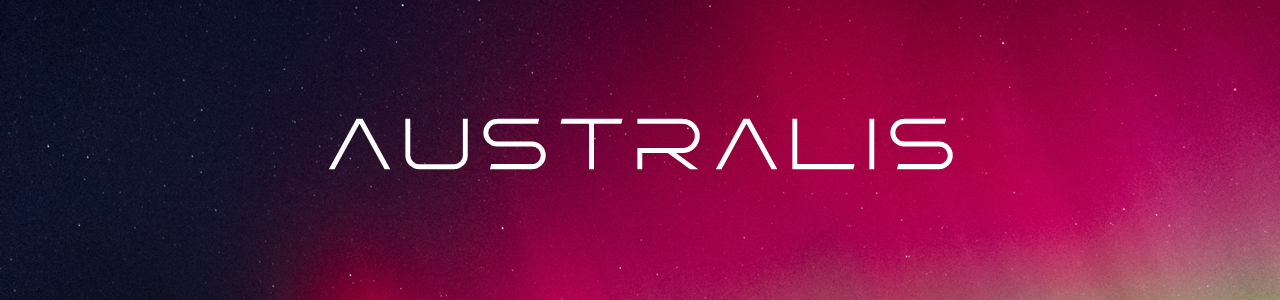
\includegraphics[width=\paperwidth]{./img/banner.png}}

  \section*{\hspace{-\margindedent}Introduction}
  This document servers to provide a comprehensive overview of the Australis Firmware system architecture and its implementation.
  
  \section*{\hspace{-\margindedent}Related Documents}
  Available from \url{https://github.com/RMIT-Competition-Rocketry/}:
  \vspace{-0.5em}
  \begin{itemize}
    \item AV2 Hardware Reference
  \end{itemize}
  
  \section*{\hspace{-\margindedent}Acknowledgements}
  Thank you to Aurora \& Legacy project team leads Patrick Underwood and Brodie Alexander for providing the opportunity and environment to work on these rockets as part of the team, and thank you to everyone who helped make them a reality!

  \subsection*{\hspace{-\margindedent}Key Contributors}
  Thank you to these contributors, without whom the Australis Firmware would not exist.
  \vspace{-0.5em}
  \begin{itemize}
    \setlength{\itemindent}{2em}
    \item Matthew Ricci     -- \textit{Principal firmware developer}
    \item William Houlahan  -- \textit{Initial driver implementations}
    \item Benjamin Wilsmore -- \textit{Initial driver implementations}
  \end{itemize}

  \subsection*{\hspace{-\margindedent}Special Thanks}
  
  Other members of the Aurora V Avionics team:
  \vspace{-0.5em}
  \begin{itemize}[]
    \setlength{\itemindent}{2em}
    \item Hugo Begg -- \textit{avionics hardware}
    \item Jonathan Chandler -- \textit{ground control station}
    \item Jeremy Timotius -- \textit{data analysis}
    \item Lucas Webb -- \textit{ground control station}
  \end{itemize}

  \clearpage

  % ----------------------------------------------------------------------------------

  % DOCUMENT INFO
  % ----------------------------------------------------------------------------------
  
  \vspace*{\fill}
  
  % TITLE
  \titleAM{\sysname}{\docname}
  \documentInfo{1.0}{\DTMdate{2025-03-11}}

  \vspace*{\fill}
  
  %     This is for adding any document content unrelated to title/contents pages 
  % ⌄⌄⌄ to place before the table of contents itself
  \clearpage
  \input{precontent}
  \clearpage
  
  % ----------------------------------------------------------------------------------

  % CONTENTS
  \tableofcontents*
  \thispagestyle{ruled}

  % MAIN DOCUMENT
  \clearpage
  \markboth{}{}
  \pagestyle{ruled}

\phantomsection
\section*{Important Terms}
\addcontentsline{toc}{section}{Important Terms}
\begin{description}[leftmargin=8em,style=multiline]
    \item[Australis] SRAD flight computer platform for high power rockets.
    \item[Australis Core] An internal component providing the base API and critical logic; stylised as \verb|core|.
    \item[Australis Extra] An internal component providing modular systems that may be optionally included to extend core functionality; stylised as \verb|extra|.
    \item[Australis Firmware] Flight computer firmware system for high power rockets; designed for, but not limited to, deployment on Australis targets.
    \item[Component] A collection of semantically related code groups and files within the Australis Firmware ecosystem.
    \item[Device] A hardware element external to the controller that provides additional functionality via a connected interface.
    \item[Driver] Software implementation of a device or peripheral interface.
    \item[Peripheral] A hardware element internal to the controller that provides important extensions to the feature set of its core processor.
    \item[Submodule] An isolated source group packaged within \verb|extra|, that extends system functionality to target code. Submodules may only depend on the \verb|core| API.
    \item[Subtarget] A single connected hardware unit as part of a target, consisting of one or more unique chain-programmable controllers.
    \item[Target] A hardware platform on which the Australis Firmware operates.
\end{description}

\phantomsection
\section*{Abbreviations}
\addcontentsline{toc}{section}{Abbreviations}
\begin{description}[leftmargin=4em,style=multiline]
    \item[A3\footnotemark] Aurora 3
    \item[API] Application Programming Interface
    \item[AV2] Australis Version 2
    \item[COTS] Commercial Off The Shelf
    \item[SRAD] Student Researched And Developed
\end{description}
\footnotetext{{Also refers to version 1 of the Australis flight computer hardware.}}

\clearpage


\section{System Overview}

\begin{tcolorbox}[colback=red!5, breakable, enhanced]
\paragraph{\color{red}A Note on Endianness}\mbox{} \\[0.5em]
All data in this document is presented in Big-endian notation, unless otherwise specified.\\[0.5em]
In reference to byte order, this means that the lower address of a datum represents the least significant byte of the complete value.
\end{tcolorbox}

\subsection{Firmware Architecture}
Australis Firmware is a software platform for implementing FreeRTOS task systems designed for high power rockets based on STM32 hardware. It is packaged as two internal components, \verb|core| and \verb|extra|, which can be integrated by developers to create a complete flight computer system for their required target.

\begin{figure}[h]
    \centering
    \begin{tikzpicture}
        % Core ------------------------------------------------------------------------------------
        \node[element, minimum width=8cm, fill=pastelyellow!50](core){Australis Core};
        \node[element, minimum width=3cm, above=5mm of core.north, xshift=-2.15cm, fill=pastelgreen!50](core_state){State};
        \node[element, minimum width=3cm, above=5mm of core.north, xshift=2.15cm, fill=pastelgreen!50](core_devices){Devices};
        % Core group
        \begin{pgfonlayer}{background}
            \node[second_group, fit={(core_state) (core_devices)}](group_rectangle)(inner_main_group){};
        \end{pgfonlayer}
        \begin{pgfonlayer}{subbackground}
            \node[group, fit={(inner_main_group) (core)}, minimum width=4cm](group_rectangle)(main_group){};
        \end{pgfonlayer}
        % Extra ------------------------------------------------------------------------------------
        \node[element, minimum width=3cm, above=12.5mm of core_state.north, fill=pastelyellow!50](extra){Australis Extra};
        \node[element, minimum width=3cm, above=12.5mm of core_devices.north](target){Target\footnotemark};
        % Extra group
        \begin{pgfonlayer}{background}
            \node[group, fit={(extra) (target)}, minimum width=8.5cm](group_rectangle)(extra_group){};
        \end{pgfonlayer}
        % Legend -----------------------------------------------------------------------------------
        \node[square, minimum width=4mm, anchor=north west, above=5mm of extra_group.north west, xshift=7mm, draw=black, fill=pastelyellow, label={right:Australis Firmware}](legend_firmware){};
        \node[square, minimum width=4mm, right=of legend_firmware, xshift=3cm, draw=black, fill=pastelgreen, label={right:Australis Interface}](legend_interface){};
        % Subscript --------------------------------------------------------------------------------
        \useasboundingbox (current bounding box);
        % Labels -----------------------------------------------------------------------------------
        \node[label, left=0.2cm of main_group]{Australis Core layer};
        \node[label, left=0.2cm of extra_group]{Australis Target layer};
        % Arrows -----------------------------------------------------------------------------------
        \draw[-Triangle,thick] (core_state.north) |- ([yshift=-5mm]target.south) -- (target.south);
        \draw[-Triangle,thick] (core_devices.north) |- ([yshift=-5mm]extra.south) -- (extra.south);
        \draw[Triangle-Triangle,thick] (extra.east) -- (target.west);
    \end{tikzpicture}
    \caption{Australis Firmware system architecture}
    \label{fig:architecture}
\end{figure}
\footnotetext{Target component is implementation specific.}

Australis Firmware implements a layered architecture (pictured Fig.~\ref{fig:architecture}), where \verb|core| defines the base which provides the system API and critical logic, with the target layer on top integrating both \verb|extra| submodules and target source code.

\subsection{Components}

\subsubsection{Core}
\paragraph{State}
\paragraph{Devices}

\subsubsection{Extra}

\subsection{Data Storage and Interpretation}
Data is stored in hardware-provided external flash as a series of dataframes which indicate the type of data and its contents. At present, there are three key dataframes that are defined: 

\vspace{-0.5em}
\begin{itemize}
    \item \textbf{High resolution data} contains the raw data collected from the high resolution sensors (accelerometers, gyroscope)
    \item \textbf{Low resolution data} contains the raw data collected from the low resolution sensors (barometer)
    \item \textbf{Event timestamps} contain an event identifier (e.g. apogee reached) and a time-of-flight millisecond counter to provide timing information for post-flight analysis
\end{itemize}

These dataframes are organised by header and payload, as described in Figure~\ref{fig:dataframe-structure}, where frame headers define the boundaries of each payload.

\begin{figure}[h!]
  \begin{center}\hspace{4.5em}
  \begin{bytefield}[bitwidth=2em, endianness=big]{8}
    \bitheader{0,7}\\
    \begin{rightwordgroup}{Header}
      \wordbox{1}[bgcolor=aquamarine]{ID}\\
      \wordbox{1}[bgcolor=lavender]{Payload Length} \\
      \wordbox{1}[bgcolor=lavender]{Payload CRC$_{[15:8]}$} \\
      \wordbox{1}[bgcolor=lavender]{Payload CRC$_{[7:0]}$} 
    \end{rightwordgroup}\\
    \begin{rightwordgroup}{Payload}
      \wordbox{1}{$D_0$}\\
      \wordbox{1}{$D_1$}\\
      \wordbox[lrt]{1}{}\\
      \cskippedwords{blue!20}\\
      \wordbox[lrb]{1}{}\\
      \wordbox{1}{$D_n$}
    \end{rightwordgroup}
  \end{bytefield}
  \end{center}
  \caption{Dataframe structure for avionics}
  \label{fig:dataframe-structure}
\end{figure}

A dataframe header consists of four bytes. The first byte defines the frame identifier, indicating the type of dataframe. The second byte defines the payload length, which describes how many bytes are contained within the payload of the dataframe.

The last two bytes in the header contain a CRC encoding of the payload data. This allows for post-processing analysis to better identify and reject invalid or corrupt data.

\subsubsection{Interpreting Binary Data}

Algorithm~\ref{alg:dataframe-validation} provides a simple, pseudocode defined implementation for dataframe validation when performing post-flight data analysis.

This approach simply iterates through every byte of data retrieved from the binary, extracts the bytes that \textit{would} contain the payload length and CRC in a valid dataframe, and compares the expected CRC to the calculated CRC of the assumed payload.

\settowidth{\LHSwidth}{\mbox{\ttfamily$\text{length}_{[0]}$}}

\begin{algorithm}[alg:dataframe-validation]{Simple dataframe validation}
(!\textit{Assume \emph{\bfseries crc16} is a function that accepts some arbitrary binary series and its length, and returns its 16-bit CRC encoding.}!)

input:  (!An array of 8-bit binary values, \emph{data}!) 
output: (!A valid data payload!)

foreach byte in (!\emph{data}!) do:
    (!\LHS{$\text{id}_{[0]}$}!) <- $\ast$(byte)
    (!\LHS{$\text{length}_{[0]}$}!) <- $\ast$(byte + 1)
    (!\LHS{$\text{crc}_{[1:0]}$}!) <- $\ast$(byte + 2)

    payload <- (byte + 4)

    if crc is (!\emph{\bfseries crc16(payload, length)}!) then:
        return payload

    else: continue
\end{algorithm}

Full implementation details are beyond the scope of this document and may not entirely pertain to the definition of Algorithm~\ref{alg:dataframe-validation}. 

More efficient methods of analysis are possible, this simply serves as a high level informational breakdown of the process of interpreting the binary data.

\section{Implementation Details}

\section{Future Progress}

\begin{figure}[ht]
    \centering
    \begin{tikzpicture}
        \node[element, minimum width=8.5cm, fill=pastelyellow!50](portable){Australis Portable};
        % Core ------------------------------------------------------------------------------------
        \node[element, minimum width=8cm, above=8mm of portable.north, fill=pastelyellow!50](core){Australis Core};
        \node[element, minimum width=3cm, above=5mm of core.north, xshift=-2.15cm, fill=pastelgreen!50](core_state){State};
        \node[element, minimum width=3cm, above=5mm of core.north, xshift=2.15cm, fill=pastelgreen!50](core_devices){Devices};
        % Core group
        \begin{pgfonlayer}{background}
            \node[second_group, fit={(core_state) (core_devices)}](group_rectangle)(inner_main_group){};
        \end{pgfonlayer}
        \begin{pgfonlayer}{subbackground}
            \node[group, fit={(inner_main_group) (core)}, minimum width=4cm](group_rectangle)(main_group){};
        \end{pgfonlayer}
        % Extra ------------------------------------------------------------------------------------
        \node[element, minimum width=3cm, above=12.5mm of core_state.north, fill=pastelyellow!50](extra){Australis Extra};
        \node[element, minimum width=3cm, above=12.5mm of core_devices.north](target){Target};
        % Extra group
        \begin{pgfonlayer}{background}
            \node[group, fit={(extra) (target)}, minimum width=8.5cm](group_rectangle)(extra_group){};
        \end{pgfonlayer}
        % Legend -----------------------------------------------------------------------------------
        \node[square, minimum width=4mm, anchor=north west, above=5mm of extra_group.north west, xshift=7mm, draw=black, fill=pastelyellow, label={right:Australis Firmware}](legend_firmware){};
        \node[square, minimum width=4mm, right=of legend_firmware, xshift=3cm, draw=black, fill=pastelgreen, label={right:Australis Interface}](legend_interface){};        \useasboundingbox (current bounding box);
        % Labels -----------------------------------------------------------------------------------
        \node[label, left=0.2cm of portable]{Australis portable layer};
        \node[label, left=0.2cm of main_group]{Australis Core layer};
        \node[label, left=0.2cm of extra_group]{Australis Target layer};
        % Arrows -----------------------------------------------------------------------------------
        \draw[-Triangle,thick] (core_state.north) |- ([yshift=-5mm]target.south) -- (target.south);
        \draw[-Triangle,thick] (core_devices.north) |- ([yshift=-5mm]extra.south) -- (extra.south);
        \draw[Triangle-Triangle,thick] (extra.east) -- (target.west);
    \end{tikzpicture}
    \caption{Proposed system architecture}
    \label{fig:architecture_portable}
\end{figure}



  % REFERENCES
  \renewcommand*{\UrlFont}{\rmfamily}
  \printbibliography[heading=references]
  \clearpage
  
  % CHANGELOG
  \section{Document History}
  \begin{table}[h]
  \centering
  \centerline{\begin{tabularx}{\headwidth}{lll}
  Date & Changes Made & Made By \\
  \midrule
  \DTMdisplaydate{2025}{03}{16}{-1} & Create initial document & Matthew Ricci\\
  \midrule
  \end{tabularx}}
  \end{table}  

  % APPENDIX
  \clearpage
  \sectionmark{Appendix}
\phantomsection
\section*{Appendix}
\addcontentsline{toc}{section}{\hspace{\tocsecnumwidth}Appendix}

\setsecnumformat{Appendix \csname the#1\endcsname:\ }
\renewcommand{\thesubsection}{\Alph{subsection}}
\renewcommand{\thefigure}{\Alph{subsection}.\arabic{figure}}

\subsection{Appendix Item}

\clearpage


\end{document}
